% Version 1.2 of SN LaTeX, November 2022
%
% See section 11 of the User Manual for version history 
%
%%%%%%%%%%%%%%%%%%%%%%%%%%%%%%%%%%%%%%%%%%%%%%%%%%%%%%%%%%%%%%%%%%%%%%
%%                                                                 %%
%% Please do not use \input{...} to include other tex files.       %%
%% Submit your LaTeX manuscript as one .tex document.              %%
%%                                                                 %%
%% All additional figures and files should be attached             %%
%% separately and not embedded in the \TeX\ document itself.       %%
%%                                                                 %%
%%%%%%%%%%%%%%%%%%%%%%%%%%%%%%%%%%%%%%%%%%%%%%%%%%%%%%%%%%%%%%%%%%%%%

%%\documentclass[referee,sn-basic]{sn-jnl}% referee option is meant for double line spacing

%%=======================================================%%
%% to print line numbers in the margin use lineno option %%
%%=======================================================%%

%%\documentclass[lineno,sn-basic]{sn-jnl}% Basic Springer Nature Reference Style/Chemistry Reference Style

%%======================================================%%
%% to compile with pdflatex/xelatex use pdflatex option %%
%%======================================================%%

%%\documentclass[pdflatex,sn-basic]{sn-jnl}% Basic Springer Nature Reference Style/Chemistry Reference Style


%%Note: the following reference styles support Namedate and Numbered referencing. By default the style follows the most common style. To switch between the options you can add or remove �Numbered� in the optional parenthesis. 
%%The option is available for: sn-basic.bst, sn-vancouver.bst, sn-chicago.bst, sn-mathphys.bst. %  
 
%%\documentclass[sn-nature]{sn-jnl}% Style for submissions to Nature Portfolio journals
%%\documentclass[sn-basic]{sn-jnl}% Basic Springer Nature Reference Style/Chemistry Reference Style
\documentclass[sn-mathphys, Numbered]{sn-jnl}% Math and Physical Sciences Reference Style
%%\documentclass[sn-aps]{sn-jnl}% American Physical Society (APS) Reference Style
%%\documentclass[sn-vancouver,Numbered]{sn-jnl}% Vancouver Reference Style
%%\documentclass[sn-apa]{sn-jnl}% APA Reference Style 
%%\documentclass[sn-chicago]{sn-jnl}% Chicago-based Humanities Reference Style
%%\documentclass[default]{sn-jnl}% Default
%%\documentclass[default,iicol]{sn-jnl}% Default with double column layout

%%%% Standard Packages
%%<additional latex packages if required can be included here>

\usepackage{graphicx}%
\usepackage{multirow}%
\usepackage{amsmath,amssymb,amsfonts}%
\usepackage{amsthm}%
\usepackage{hhline} 
\usepackage{mathrsfs}%
\usepackage[title]{appendix}%
\usepackage{xcolor}%
\usepackage{textcomp}%
\usepackage{manyfoot}%
\usepackage{booktabs}%
\usepackage{algorithm}%
\usepackage{algorithmicx}%
\usepackage{algpseudocode}%
\usepackage{listings}%
\usepackage[compatibility=false]{caption}
\usepackage{caption}
\usepackage{lipsum}                     % Dummytext
\usepackage{xargs}                      % Use more than one optional parameter in a new commands
%\usepackage{courier}
%  \usepackage[
%backend=biber,
%style=stylename,
%]{biblatex}
\usepackage[colorinlistoftodos,prependcaption,textsize=tiny]{todonotes}
\newcommandx{\unsure}[2][1=]{\todo[linecolor=red,backgroundcolor=red!25,bordercolor=red,#1]{#2}}
\newcommandx{\change}[2][1=]{\todo[linecolor=blue,backgroundcolor=blue!25,bordercolor=blue,#1]{#2}}
\newcommandx{\info}[2][1=]{\todo[linecolor=OliveGreen,backgroundcolor=OliveGreen!25,bordercolor=OliveGreen,#1]{#2}}
\newcommandx{\improvement}[2][1=]{\todo[linecolor=Plum,backgroundcolor=Plum!25,bordercolor=Plum,#1]{#2}}
\newcommandx{\thiswillnotshow}[2][1=]{\todo[disable,#1]{#2}}
% \addbibresource{sn-bibliography}
 
\lstdefinelanguage{Muesli}
{
	language=C,
	% list of keywords
	basicstyle=\ttfamily,
	keywordstyle = {\color{violet}\bfseries},
	keywordstyle = [2]{\color{purple}\bfseries},
	keywordstyle = [3]{\color{magenta}\bfseries},
	keywordstyle = [4]{\color{blue}\bfseries},
	otherkeywords = {},%{;,<<,>>,++,+=,=,<,>, int, config},
	morekeywords = [2]{},%;,=,<,>},
tabsize=2,
morekeywords = [4]{Functor2,Functor4,MSL_USERFUNC},
morekeywords = [4]{mapStencilMM,DA,DC,DM,fold, mapIndex,mapIndexInPlace,zipInPlace,zip,DMMapStencilFunctor, PLATFORM, GPU, CPU_MPMD, PROCESSES, GPUS, MODE, release, CORES, roi_start, roi_end, PLCube, MapStencilKernelDC, DCMapStencilFunctor, mapStencil, mapStencilKernelDC, Muesli },
basicstyle = {\ttfamily \color{darkgray}},
numberstyle=\color{darkgray},
numbers=left,
belowcaptionskip=0.5em,
belowskip=0.1em,
%backgroundcolor = {\color{back-color}},
stringstyle = {\color{darkgray}},
sensitive=true, % keywords are not case-sensitive
morecomment=[l]{//}, % l is for line comment
morecomment=[s]{/*}{*/}, % s is for start and end delimiter
morekeywords = [1]{template, size_t, int, float, for, return, else, ifdef, endif, pragma, omp, parallel},
morestring=[b]", % defines that strings are enclosed in double quotes
showspaces=false,                
showstringspaces=false
}
%%%%

%%%%%=============================================================================%%%%
%%%%  Remarks: This template is provided to aid authors with the preparation
%%%%  of original research articles intended for submission to journals published 
%%%%  by Springer Nature. The guidance has been prepared in partnership with 
%%%%  production teams to conform to Springer Nature technical requirements. 
%%%%  Editorial and presentation requirements differ among journal portfolios and 
%%%%  research disciplines. You may find sections in this template are irrelevant 
%%%%  to your work and are empowered to omit any such section if allowed by the 
%%%%  journal you intend to submit to. The submission guidelines and policies 
%%%%  of the journal take precedence. A detailed User Manual is available in the 
%%%%  template package for technical guidance.
%%%%%=============================================================================%%%%

%\jyear{2021}%

%% as per the requirement new theorem styles can be included as shown below
\theoremstyle{thmstyleone}%
\newtheorem{theorem}{Theorem}%  meant for continuous numbers
%%\newtheorem{theorem}{Theorem}[section]% meant for sectionwise numbers
%% optional argument [theorem] produces theorem numbering sequence instead of independent numbers for Proposition
\newtheorem{proposition}[theorem]{Proposition}% 
%%\newtheorem{proposition}{Proposition}% to get separate numbers for theorem and proposition etc.
\usepackage[nolist,nohyperlinks]{acronym}

\theoremstyle{thmstyletwo}%
\newtheorem{example}{Example}%
\newtheorem{remark}{Remark}%

\theoremstyle{thmstylethree}%
\newtheorem{definition}{Definition}%
\newcommand{\RN}[1]{\uppercase\expandafter{\romannumeral#1}}
\raggedbottom
%%\unnumbered% uncomment this for unnumbered level heads

\begin{document}

\begin{acronym}[ACO]
	\acro{muesli}[Muesli]{Muenster Skeleton Library}
	\acro{hpc}[HPC]{High Performance Computing}
	\acro{dsl}[DSL]{domain-specific language}
	\acro{dc}[DC]{distributed cube}
	\acro{gpu}[GPU]{graphics processing unit}
	\acro{mpi}[MPI]{Message Passing Interface}
	\acro{lbm}[LBM]{Lattice Boltzmann method}
	\acro{cpu}[CPU]{central processing unit}
	%s\acroplural{cpu}[CPUs]{Computational processing units}
\end{acronym}
\title[Article Title]{Optimizing Three-Dimensional Stencil-Operations on Heterogeneous Computing Environments}

%%=============================================================%%
%% Prefix	-> \pfx{Dr}
%% GivenName	-> \fnm{Joergen W.}
%% Particle	-> \spfx{van der} -> surname prefix
%% FamilyName	-> \sur{Ploeg}
%% Suffix	-> \sfx{IV}
%% NatureName	-> \tanm{Poet Laureate} -> Title after name
%% Degrees	-> \dgr{MSc, PhD}
%% \author*[1,2]{\pfx{Dr} \fnm{Joergen W.} \spfx{van der} \sur{Ploeg} \sfx{IV} \tanm{Poet Laureate} 
%%                 \dgr{MSc, PhD}}\email{iauthor@gmail.com}
%%=============================================================%%

\author*[1]{\fnm{Nina} \sur{Herrmann}}\email{nina.herrmann@uni-muenster.de}
\equalcont{These authors contributed equally to this work.}

\author[1]{\fnm{Justus} \sur{Dieckmann}}\email{justus.dieckmann@uni-muenster.de}
\equalcont{These authors contributed equally to this work.}

\author[1]{\fnm{Herbert} \sur{Kuchen}}\email{kuchen@uni-muenster.de}


\affil*[1]{\orgdiv{Practical Computer Science}, \orgname{University of M\"{u}nster}, \orgaddress{\street{Leonardo-Campus 3}, \city{M\"{u}nster}, \postcode{48149}, \country{Germany}}}


%%==================================%%
%% sample for unstructured abstract %%
%%==================================%%

\abstract{Complex algorithms and enormous data sets require parallel execution of programs to attain results in a reasonable amount of time. Both aspects are combined in the domain of three-dimensional stencil operations, for example, computational fluid dynamics. This work contributes to the research on high-level parallel programming by discussing the generalizable implementation of a three-dimensional stencil skeleton that works in heterogeneous computing environments. Two exemplary programs, a gas simulation with the Lattice Boltzmann method, and a mean blur, are executed in a multi-node multi-\acp{gpu} environment, proving the runtime improvements in heterogeneous computing environments.}

%%================================%%
%% Sample for structured abstract %%
%%================================%%

% \abstract{\textbf{Purpose:} The abstract serves both as a general introduction to the topic and as a brief, non-technical summary of the main results and their implications. The abstract must not include subheadings (unless expressly permitted in the journal's Instructions to Authors), equations or citations. As a guide the abstract should not exceed 200 words. Most journals do not set a hard limit however authors are advised to check the author instructions for the journal they are submitting to.
% 
% \textbf{Methods:} The abstract serves both as a general introduction to the topic and as a brief, non-technical summary of the main results and their implications. The abstract must not include subheadings (unless expressly permitted in the journal's Instructions to Authors), equations or citations. As a guide the abstract should not exceed 200 words. Most journals do not set a hard limit however authors are advised to check the author instructions for the journal they are submitting to.
% 
% \textbf{Results:} The abstract serves both as a general introduction to the topic and as a brief, non-technical summary of the main results and their implications. The abstract must not include subheadings (unless expressly permitted in the journal's Instructions to Authors), equations or citations. As a guide the abstract should not exceed 200 words. Most journals do not set a hard limit however authors are advised to check the author instructions for the journal they are submitting to.
% 
% \textbf{Conclusion:} The abstract serves both as a general introduction to the topic and as a brief, non-technical summary of the main results and their implications. The abstract must not include subheadings (unless expressly permitted in the journal's Instructions to Authors), equations or citations. As a guide the abstract should not exceed 200 words. Most journals do not set a hard limit however authors are advised to check the author instructions for the journal they are submitting to.}

\keywords{Skeleton Programming, Three-Dimensional Stencil Operations}

%%\pacs[JEL Classification]{D8, H51}

%%\pacs[MSC Classification]{35A01, 65L10, 65L12, 65L20, 65L70}

\maketitle

\section{Introduction}\label{sec1}

The field of \ac{hpc} is growing as algorithms become more complex and more data is available. Evaluating massive datasets, therefore, requires writing efficient parallel programs. Most \ac{hpc} environments have multiple nodes equipped with multiple \acp{cpu} and \acp{gpu}. Creating programs which combine multiple types of hardware requires knowledge of low-level frameworks such as \ac{mpi} \citep{MPI}, OpenMP \citep{OpenMP}, and CUDA \citep{CUDA}. Writing a parallel program is error prone and tedious as e.g. out of memory errors, and invalid memory accesses are troublesome to identify even for skilled programmers. Moreover, choosing memory spaces, distributing data, and assigning task to threads are design decision which have a high impact on performance but require experience. Writing a program which combines multiple frameworks overstrains scientist.

Since experts in this field are hard to find, high-level frameworks are often used. Those frameworks commonly abstract from the distribution of data, provide portable code for different hardware architecture, are adjustable to distinct accelerators, and require less maintainance for the end-user. In 1989 \textsc{Cole} introduced algorithmic skeletons, enclosing reoccurring parallel and distributed computing patterns, such as Map and Reduce as one of the most common approaches to abstract from low-level details \cite{cole1989}. Multiple libraries \cite{ernsting2017,benoit2005}, general frameworks \cite{ernstsson2021skepu,fastflowmulticore}, and and \acp{dsl}\cite{Wrede2019} utilize the concept. 

The paper contributes to the ongoing work by focusing on a particularly arduous operation, namely three-dimensional stencil operations. Stencil operations calculate elements depending on other values inside the data structure and therefore require communication between the computational units used. Those operations are irreplaceable, for e.g., simulation of gas or computational fluid dynamics.
Efficiently updating data in a generalizable way and dealing with 3D data structures are obstacles not solved in current high-level approaches.

This paper firstly elaborates on the related work, focusing on high-level approaches abstracting from problem specific details (Section \ref{sec:relatedwork}). Section \ref{sec:muesli} outlines the library used (muesli), while Section \ref{sec:newmuesli} explains the additional implementation of the three-dimensional skeleton. The work is evaluated in Section \ref{sec:evaluation} discusing our runtime experiments on multiple hardware set-ups. Lastly, Section \ref{sec:conclusion} summarizes out work. 

% \cite{ernsting2012,ernsting2017,benoit2005}, \acp{dsl} \cite{Wrede2019}, and general frameworks \cite{ernstsson2021skepu,aldinucci2017fastflow}.


\section{Related Wok}\label{sec:relatedwork}

Ongoing work discussing three-dimensional stencil operations is twofold. On the one hand, there exist generic high-level frameworks which have the advantage of parallelizing pre- and postprocessing steps, as many of them offer a variety of operations/skeletons. On the other hand, specialized frameworks already contain algorithms' implementations but are often inefficient. 
Most related regarding high-level skeleton programming, SkePU3 targets multi-node and multi-\ac{gpu} environments for most skeletons in combination with StarPU. However, for stencil operations (MapOverlap), the exchange of data between the programs is missing for multi-node programs \cite{ernstsson2021skepu}. FastFlow added \ac{gpu} support but focuses on communication skeletons and misses a comparable stencil operation \cite{fastflowhetogeneous}\cite{fastflowmulticore}. 

Specialized libraries such as Palabos for the \acp{lbm} \cite{boltzmannpalabos}, or publications discussing a single method, e.g., the  Helmholtz equation \cite{fftparallel} focus rather on the algorithm and do not include accelerators as \acp{gpu}, which provide a significant speed-up.
 
This work extends the mentioned work as the presented stencil skeleton is generalizable for multiple methods and abstracts from the multiple layers of parallelism. This is profen by showing the implementation of a \ac{lbm} and a three-dimensional mean blur. Both programs run on multiple nodes and with multiple \acp{gpu}.

\section{The {\it Mue}nster {\it S}keleton {\it Li}brary {\it Muesli}}\label{sec:muesli}
Skeleton Programming is mostly present in functional languages since it originates from functional languages \cite{cole1989}. Most of the frameworks are implemented in C/C++ \cite{ernstsson2021skepu, fastflowmulticore,benoit2005, marrow, mallba, Sketo}, as it offers interoperability with multiple parallel frameworks such as OpenMP, \ac{mpi}, CUDA, and OpenCL and is exceptionally performant. Noteworthy, Python recently gained attention for natural science applications as it provides a easy interface to write packages in C/C++ which can provide roughly the same performance as C/C++ programs. However, those packages are very specialized as custom user can only be passed with a overhead decreasing the runtime. Therefore, especially in the \ac{hpc} environment C/C++ is the first choice.

The used library is called \ac{muesli}. \ac{muesli} provides an object-oriented approach offering one, two and three-dimensional datastructures (DA, DM, DC) which call skeletons as member functions. The supported skeletons are for example multiple version of Map and Zip (index and inplace variants), Fold, Gather, and as discussed in this work MapStencil. Internally, , \ac{mpi}, OpenMP, and CUDA are used, which enables simultaneously parallelism on multiple nodes, \acp{cpu}, annd \acp{gpu}. The library can be included with a simple include statement \verb|#include<muesli.h>|. For writing a parallel program, muesli provides abstract methods to state the number of processes and \acp{gpu} used. Apart from that \ac{muesli} abstracts from parallel programming details by internally distributing the datastructures on the available computational units, choosing the number of threads started on the corresponding low-level framework and copying data to the correct memory spaces. This abstraction has the additional effect to reduce errors which are commonly made by inexperienced programmers such as race conditions and inefficient data distribution. 

Listing \ref{lst:examplemuesli} shows a simple program calculating the Scalar product of the distributed arrays a and b. In line 6 a distributed array of size three with a default value of 2 is created. In the skeleton calls in line 7-9 can be seen that skeletons have a user function as an argument which can either be a C++ function or a C++ functor. For the \verb|index| variant in line 7 \ac{muesli} complements the missing arguments internally. For the \verb|zip| skeleton the second required data structure is also passed as an argument. Lastly, l.7+9 show das function can be used in differnt context, firstly for calculating the sum of the index and the value and secondly as a reduction operator.
\lstset{language=muesli}        
\begin{lstlisting}[basicstyle=\small, language=muesli, caption={Scalar product in Muesli}, label=lst:examplemuesli]
class Sum : public Functor2<int, int, int>{
	public: MSL_USERFUNC int operator() (int x, int y) 
	const {return x+y;}};
Sum sum;
auto product = [] (int i, int j) {return i*j;};
DA<int> a(3,2);                     // delivers: {2,2,2}
DA<int> b = a.mapIndex(sum);        // delivers: {2,3,4}
a.zipInPlace(b,product);            // delivers: {4,6,8}
int scalarproduct = a.fold(sum);    // delivers: 18
\end{lstlisting}

\section{Three-Dimensional Stencil Operations}\label{sec:newmuesli}
\begin{wrapfigure}{r}{0.25\textwidth}
	\centering
	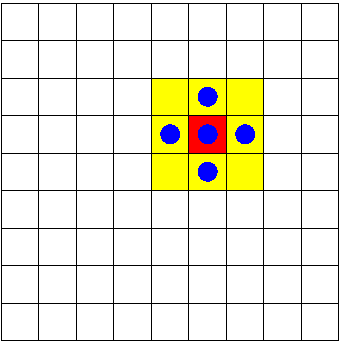
\includegraphics[width=0.25\textwidth]{stencil.pdf}
	\caption{Stencil Operation}\label{fig:stencil}
\end{wrapfigure}
Stencil operations are map operation which additionally require to read the surrounding elements of the datastructure. 
Figure \ref{fig:stencil} displays a two-dimensional stencil with the size one. The peculiarity regarding stencil operations on multiple nodes and accelerators is that each execution of the stencil operation requires to update elements which are shared between computational units. As communication of updated elements requires synchronization between the computational nodes it decreases the opportunity for executing task in parallel within the program.
\ac{muesli} abstracts from all communication between the computational nodes with a MapStencil Skeleton. The usage of the skeleton for the end-user is shown in Listing \ref{lst:stencilmuesli}. 

\subsection{Using the MapStencil Skeleton}
Firstly, a function which is executed on each element is defined (l. 1-12). Merely functors of type \verb|DCMapStencilFunctor| are permitted to be used with the \verb|mapStencil| skeleton. Therefore, the first argument of the functor has to of type \verb|PLCube| (\textit{PaddedLocalCube}), and the following arguments have to be integers for indexing the data structure. The class \verb|PLCube| most importantly offers a getter taking three index arguments, relieving the end-user from index calculations (l.9). The presented functor calculates the sum of all elements with a radius of two and divides the sum with the number of total elements, therefore calculating a mean blur. This functor can be applied to a distributed cube by calling the mapStencil skeleton as a member function (l.19). The skeleton takes the functor as a template argument, and requires a distributed cube of the same dimension with the current data \footnote{A variant of the skeleton which immediately overwrites old values by new values is however possible and could be applied,
	for instance, for implementing the Gau{\ss}-Seidel method for solving systems of linear equations.}, the radius of the stencil\footnote{Other stencil shapes such as rectangular or irregular stencils can be handled by using the smallest surrounding square, although this may introduce some overhead.} and the neutral value for border elements. 
\lstset{language=muesli}        
\begin{lstlisting}[language=muesli, caption={Exemplary Functor for Stencil Skeleton}, label=lst:stencilmuesli]
MSL_USERFUNC float update(const PLCube<float> &plCube, 
						  int x, int y, int z) {
	float res = 0;
	const int radius = 2;
	const int elements = 48;
	for (int mx = x - radius; mx <= x + radius; mx++) {
		for (int my = y - radius; my <= y + radius; my++) {
			for (int mz = z - radius; mz <= z + radius; mz++) {
				res += plCube(mx, my, mz);
			}
		}
	}
	return res/(elements);
}
...
main () {
	...
	int stencilradius = 2;
	dcp1->mapStencil<update>(*dcp2, stencilradius, 0);
	...
}
\end{lstlisting}

\subsection{Implementation of the MapStencil Skeleton}
Adding the MapStencil skeleton to the existing \ac{dc} class requires to add two additional parameters: a vector of \verb|PLCubes| and a supported stencil size. As previously mentioned the \verb|PLCubes| class serves for the end-user to abstract from indexing of the datastructure. To make the access to the different memory spaces efficient each computational unit has a separate \verb|PLCubes| storing merely the elements needed for the calculations of the assigned elements. This design choice makes the class flexible to be used for \acp{cpu} as well as for \acp{gpu}. It contains the following attributes to provide a light, minimal design:
\begin{itemize}
	  \setlength\itemsep{0.2em}
	\item \verb|int width, height, depth| the three dimensions of the datastructure,
	\item \verb|int stencilSize| size of the Stencil required to calculate the overlapping elements,
	\item \verb|int neutralValue| used when the index is outside the data structure,
	\item \verb|T * data, T* topPadding, T* bottomPadding| \ac{cpu} or \ac{gpu} pointer for current data,
	\item four integers to save global indexes for start and end of datastructure and stencil size.
\end{itemize}
Most importantly, the index operator is implemented, taking three integers as arguments returning suitable value. This is either the neutral value or the corresponding element from the \ac{cpu} or \ac{gpu} memory. 

Assuming \acp{gpu} are used a s accelerators, the skeleton updates the current datastructure in case the data is not up to date (Listing \ref{lst:MapStencilImpl} l.6). Afterwards, it synchronizes the \verb|PLCubes| inside one node, and the data between multiple nodes (l.7, l.9). Foreach \ac{gpu} used the mapStencilKernelDC is called executing the functor on the appropiate part of the overall datastructure. In any other case (multiple nodes and cpu) it is only necessary to synchronize the nodes (l. 21), and thereafter call the functor with the corresponding arguments.
\begin{lstlisting}[language=muesli, caption={Implementation of MapStencil Skeleton}, label=lst:MapStencilImpl]
template<typename T>
template<msl::DCMapStencilFunctor<T> f>
void msl::DC<T>::mapStencil(msl::DC<T> &result, size_t stencilSize, 
							T neutralValue) {
	#ifdef __CUDACC__
	this->updateDevice();
	syncPLCubes(stencilSize, neutralValue);
	msl::syncStreams();
	syncPLCubesMPI(stencilSize);
	for (int i = 0; i < this->ng; i++) {
		cudaSetDevice(i);
		dim3 dimBlock(Muesli::threads_per_block);
		dim3 dimGrid((this->plans[i].size + dimBlock.x - 1) / dimBlock.x);
		detail::mapStencilKernelDC<T, f><<<dimGrid, dimBlock, 0, 
			Muesli::streams[i]>>>(result.plans[i].d_Data, this->plCubes[i], 
			result.plans[i].size);
	}
	msl::syncStreams();
	result.setCpuMemoryInSync(false);
	#else
	syncPLCubesMPI(stencilSize);
	#ifdef _OPENMP
	#pragma omp parallel for
	#endif
	for (int k = 0; k < this->nLocal; k++) {
		int l = (k + this->firstIndex) / (ncol*nrow);
		int j = ((k + this->firstIndex) - l*(ncol*nrow)) / ncol;
		int i = (k + this->firstIndex) % ncol;
		result.localPartition[k] = f(this->plCubes[0], i, j, l);
	}
	#endif
}
\end{lstlisting}


\subsection{Example Application for Three-Dimensionl Stencil Operations}
For the evaluation of our implementation two examples where used: a \ac{lbm} implementation and a mean blur. The exeamplary user function of the mean blur was already shown in Listing \ref{lst:stencilmuesli}. However, the implementation of a \ac{lbm} underlines the applicability for real application contexts.

\acp{lbm} are used for fluid simulations. It distinguishes between the collision and the streaming step which alternate in continuous simulations \cite[p.61ff]{LBMBook}. In the streaming step particles move from one cell to another. In the collision step the fluid flow caused by the colliding particles is calculated.
The distribution function $f_i(x, t)$ calculates for a cell $x$ and a timestamp $t$ how many particles move in the next step to the neighbour $i$.
Zero is the cell itself. 
\begin{equation}
	f_i(x + c_i \Delta t, t + \Delta t) := f_i^*(x, t)
\end{equation}

For the collision steps the Bhatnagar-Gross-Krook-operator is used. $f_i^*$ defines the distribution after the collission of the particles, $\Delta t$ the time period to be simulated and $\tau$ a constant defining the convergence of the simulation. Thus $\tau$ influences the viscosity of the gases.
\begin{equation}
	f_i^*(x, t) := f_i(x, t) - \frac{\Delta t}{\tau} \left( f_i(x, t) - f_i^{\textrm{eq}}(x, t) \right).
\end{equation}

The equilibrium state is calculated by
\begin{equation}
	f_i^{\textrm{eq}}(x, t) := w_i \rho \left( 1 + \frac{u \cdot c_i}{c_s^2} + \frac{u \cdot c_i}{2 c_s^4} + \frac{u \cdot u}{2 c_s^2} \right),
\end{equation}

where $w_i$ are the weights of the choosen grid and $c_i$ is the position of the neighbour cells relative to the main cell.
The constant number $c_s$ is the sound velocity of the model.
The mass density $\rho$ and the puls density $u$ are defined by

\begin{equation}
	\rho(x, t) = \sum_{i} f_i(x, t), \hspace{1cm} \rho u (x, t) := \sum_{i} c_i f_i(x, t).
\end{equation}


For the implementation of the \ac{lbm} a D3Q19-Grid was used, D being the number of dimensions and Q the number of neighbours. 
Both steps (collision and streaming) are combined in one \verb|mapStencil| call. Noteworthy, the implementation has to take into consideration that single cells can be marked as blocked, simulating objects which are barriers for the flow of air or as distributing constant velocity. Therefore, special cells are marked with \verb|Not a Number| values (Listing \ref{lst:lbm} l. 5-7). To simulate this behaviour without requiring additional storage, the handling of the floating numbers is extended. According to the IEEE-754 Standard each float has a maximal exponent with a mantisse which is not equal to zero. To identify special cells the most significant bit of the mantissa of f0 is set, so that the number is definitely understood as a
\verb|NaN|. The remaining bits of the mantissa can then be used freely to store other data. In the code, bit masks and a struct with bit-
fields are defined in the code to access this information as easily as possible (Listing \ref{lst:lbmcell}).
\begin{lstlisting}[language=muesli, caption={Handling of Barriers and Streaming Cells}, label=lst:lbmcell]
const int FLAG_OBSTACLE = 1 << 0;
const int FLAG_KEEP_VELOCITY = 1 << 1;
typedef struct {
	unsigned int mantissa : 23;
	unsigned int exponent : 8;
	unsigned int sign : 1;
} floatparts ;
\end{lstlisting}

The data stored for each cell is an \verb|array<float, Q>|. Q is a constant number for the neighbour cells an the cell itself (19). This type is appreviated in the following listing with \verb|cell_t|. Moreover, it is abstracted from the three-dimensional vector operations (l. 28,29,31,34). The user function starts by transforming the current value of the cell into the single float parts (l.4). In case we have a cell which distributes gas (\verb|FLAG_KEEP_VELOCITY|), the cell remains without changes (l.5-7). For all neighbour cells the current amount of paricles is read (l.10-12). In the collision step all cells which are obstacles reverse the flow of air (l.16-23). All other cells calculate the particles streaming from the next cells. 
\begin{lstlisting}[language=muesli, caption={Implementation of a Exemplary \ac{lbm} User Function}, label=lst:lbm]
MSL_USERFUNC cell_t update(const PLCube<cell_t> &plCube, int x, 
                           int y, int z) {
	cell_t cell = plCube(x, y, z);
	auto* parts = (floatparts*) &cell[0];
	if (parts->exponent == 255 && parts->mantissa
	    & FLAG_KEEP_VELOCITY) {
		return cell;
	}
	// Streaming.
	for (int i = 1; i < Q; i++) {
		cell[i] = plCube(x + (int) offsets[i].x, 
				y + (int) offsets[i].y, z + (int) offsets[i].z)[i];
	}
	
	// Collision.
	if (parts->exponent == 255 && parts->mantissa & FLAG_OBSTACLE) {
		if (parts->mantissa & FLAG_OBSTACLE) {
			cell_t cell2 = cell;
			for (size_t i = 1; i < Q; i++) {
				cell[i] = cell2[opposite[i]];
			}
		}
		return cell;
	}
	float p = 0;
	vec3f vp {0, 0, 0};
	for (size_t i = 0; i < Q; i++) {
		p += cell[i];
		vp += offsets[i] * cellwidth * cell[i];
	}
	vec3f v = p == 0 ? vp : vp * (1 / p);
	
	for (size_t i = 0; i < Q; i++) {
		cell[i] = cell[i] + deltaT / tau * (feq(i, p, v) - cell[i]);
	}
	return cell;
}
\end{lstlisting}

\section{Evaluation}\label{sec:evaluation}
Our approach requires to measure the speedup achieved. For this purpose the presented exemplary programs, a mean blur and a \ac{lbm} implementation were executed on the \ac{hpc} machine Palma \RN{2}\footnote{https://confluence.uni-muenster.de/pages/viewpage.action?pageId=27755336}.
Table \ref{tab:hardware} list the hardware specification of the partitions used. Those include two \ac{gpu}-partitions and one \ac{cpu}-partition. 

The gpu2080 partition is equiped with 5 nodes each with 8 GeForce RTX 2080 Ti \acp{gpu}. Complementary we used the gpuhgx partition equipped with 2 Nodes each with 8 A100 SXM \acp{gpu}. One major advantage of the Nvidia A100 SXM is that one \ac{gpu} has significantly more memory (80GB in contrast to 11GB) and more cores (6912 compared to 612). Therefore, experimenting with two partitions expands the research to proove the generalizability on varying \acp{gpu}. For testing \ac{cpu}-parallelization the zen2 partition equiped with 12 nodes with each one Zen2 (EPYC 7742) \acp{cpu} with 64 cores. To provide generalizable results, the mean runtime of 20 execution was used. For running the sequential version on the \ac{hpc}, a single Broadwell (E5-2683 v4) \ac{cpu} was used. 
\begin{table}[b]
	\resizebox{\textwidth}{!}{
		\begin{tabular}{|r||r|r|r|r|r|r|} \hline
			\multirow{+2}{*}{Identifier}& \multirow{+2}{*}{Nodes} & \multirow{+2}{*}{\ac{gpu}/\ac{cpu}-type} &\multicolumn{2}{l|}{Per Node}&\multicolumn{2}{l|}{per computational unit}\\ \hhline{~~~----}
			& & & \acp{gpu} & \acp{cpu}& storage& cores\\ \hline
			gpu2080& 5 &GeForce RTX 2080 Ti	&	8&1 &11GB&612\\  \hline
			gpuhgx&2 &Nvidia A100 SXM&8&1 &80GB&6912 \\ \hline
			zen2&12 & Zen2 (EPYC 7742) &-&128&496GB& 64\\ \hline
	\end{tabular}}
	\caption{Overview of used Hardware}
	\label{tab:hardware}
\end{table} 
Two classification numbers are particularly important for the evaluation of the programs depending on the hardware, the maximum storage and the number of cores. As can be seen in the last two columns of Table \ref{tab:hardware} the \ac{gpu} partitions vary. Therefore, experiments with the gpuhgx partition could be executed with bigger data structures, and provide a better speed-up.


\subsection{\ac{lbm} Experiment}
The \ac{lbm} is used to simulate the flow of fluid in the three dimensional space. Consequently, it is reasonable to run a experiment which does not only execute the mapSkeleton one time, but has multiple iterations simulating multiple dispersion steps. For every experiment 200 iteration were chosen to make runtimes comparable between different data sizes. 

Datasizes were chosen by exceeding the available storage. For the \ac{lbm} each cell requires 76 bytes, as each cell stores 19 32-bit floating point numbers. For the calculation a data structure to read and one to write is necessary.
 The required space for the program can be simply calculated by:
\[d(\textrm{gb}) := \sqrt[3]{\textrm{gb} \cdot \frac{2^{30}}{2 \cdot 76}}\]

This result for the RTX 2080 Ti \ac{gpu} in a maximum side length of {426}, for the A100 SXM in a side length of {826}. Although the \ac{cpu} partition would support bigger data structures the datasizes was not increased to the maximum, as the speed-up converged, and the run-time of the sequential program became unreasonable high (10 hours for calculating the \ac{lbm} simulation for a datasize of 960$^3$). 
Table \ref{tab:speedupsinglelbm} shows that for the \ac{cpu}-zen2 partition a speed-up of 116 can be reached. As the partition has 64 cores, this effect is reached by multithreading, in total 128 threads were started on the 64 cores available. In this scenario it should be considered that the calculations are easy to execute in parallel as all data resides on the memory of the single \ac{cpu} or \ac{gpu}, acccessible for all threads. In contrast, the  GeForce RTX 2080 Ti has 612 cores allowing to execute threads in parallel.
\todo[inline]{reasoning what is the maximum of threads which can be executed? what slows the application down?}
 
\begin{table}[b]
	\resizebox{\textwidth}{!}{
		\begin{tabular}{|r||r|r|r||r|r||r|r|} \hline
Datasize $^3$&seq&cpu&Speed-up&gpuhgx&speed-up&gpu2080&speed-up\\ \hline
40&1.69&0.48&3.5&0.01&141.12&0.02&75.86\\ \hline
80&15.75&0.58&27.09&0.06&275.29&0.14&115.86\\ \hline
120&56&1.3&42.96&0.18&317.67&0.44&128.28\\ \hline
160&135.61&2.02&67.19&0.41&332.04&1.14&119.4\\ \hline
\multicolumn{8}{|l|}{...}\\ \hline 
440&2994.47&30.35&98.67&8.69&344.4&21.65&\textbf{138.29}\\ \hline
\multicolumn{8}{|l|}{...}\\ \hline 
800&18572.9&173.88&106.81&52.52&\textbf{353.6}&-&- \\ \hline 
\multicolumn{8}{|l|}{...}\\ \hline 
960&34880.8&300.44&\textbf{116.1}&-&-&-&- \\ \hline
	\end{tabular}}
	\caption{Speed-up for the Parallel Implementation of the \ac{lbm} Gas Simulation for Single \ac{gpu} or \ac{cpu} Programs}
	\label{tab:speedupsinglelbm}
\end{table}

To assure that a low-level program is not significantly faster, a native implementation was programmed to be compared againt the \ac{muesli} program. Figure \ref{fig:multigpumueslinative}. As can be seen, the implementations are close to each other. In contrast to the native implementation \ac{muesli} has a slight overhead, however, as it is very small this difference is not important. Runtimes for bigger data structures are not included for one \ac{gpu} and two \acp{gpu} to increase the readbility of the graph. For two \acp{gpu} a speed-up of 1.7 compared to the single \ac{gpu} version can be achieved and for four \acp{gpu} a speed-up of 2.75 is achieved. To assure that the overhead is caused by the communication the time for the update function was measured separatly. Without the communication a speed-up of 1.94 and 3.88 was achieved which can be subscribed to the synchronization of streams. However, using multiple \acp{gpu} also has the advantage of processing bigger data structures. 
\begin{figure}[h]%
	\centering
	\includegraphics[width=0.9\textwidth]{../20801Node.png}
	\caption{Runtime comparison of a multi-\ac{gpu} \ac{muesli} program and Native Implementation of the \ac{lbm} on GeForce RTX 2080 Ti \acp{gpu}}\label{fig:multigpumueslinative}
\end{figure}
Taking multiple levels of parallelism into consideration the program is also capable to run on multiple nodes equiped with mutliple \acp{gpu}. Runtimes are depicted in Figure \ref{fig:lbmmnodemgpu}. 
\begin{table}
	\resizebox{\textwidth}{!}{
	\begin{tabular}{r||r|r|r||r|r||r|r} \hline
		Datasize $^3$&\acp{gpu} &1 N&1 N-Com&2 Ns&2 Ns -Com&Speed-up&Speed-up\\ \toprule \hline
		40&1&0.02&0.02&0.03&0.03&0.69&0.7\\ \hline
		40&2&0.03&0.02&0.1&0.02&0.34&1.24\\ \hline
		40&4&0.04&0.01&0.07&0.01&0.54&1\\ \hline \hline
		280&1&8.59&8.59&4.52&4.52&1.9&1.9\\ \hline
		280&2&5.09&4.44&3.13&2.28&1.62&1.95\\ \hline
		280&4&3.58&2.23&2.73&1.16&1.31&1.93\\  \hline \hline
		400&1&25.23&25.23&13.07&13.06&1.93&1.93\\ \hline
		400&2&14.2&12.98&8.17&6.59&1.74&1.97 \\ \hline
		400&4&9.16&6.5&6.34&3.31&1.44&1.97 \\ \botrule
	\end{tabular}}
	\caption{Speed-up for the Parallel Implementation of the \ac{lbm} Gas Simulation for Single \ac{gpu} or \ac{cpu} Programs}
	\label{tab:speedupsinglelbm}
\end{table}
\begin{table}
	\resizebox{\textwidth}{!}{
		\begin{tabular}{r||r|r r|r r|r|r} \toprule
			Datasize $^3$&\acp{gpu} &1 N&1 N-Com&4 Ns&4 Ns -Com&Speed-up&Speed-up\\ \midrule 
			40&1&0.02&0.02&0.04&0.01&0.56&2.7\\ 
			40&2&0.03&0.02&0.08&0.02&0.44&1.29\\
			40&4&0.04&0.01&0.07&0.01&0.55&0.99\\ \midrule
			280&1&8.59&8.59&2.74&2.16&3.14&3.97\\ 
			280&2&5.09&4.44&2.63&1.19&1.93&3.74\\ 
			280&4&3.58&2.23&2.06&0.39&1.73&5.74\\  \midrule 
			400&1&25.23&25.23&7.21&6.32&3.5&3.99\\ 
			400&2&14.2&12.98&6&3.35&2.37&3.87\\ 
			400&4&9.16&6.5&5.14&1.7&1.78&3.82\\ 
			\botrule
	\end{tabular}}
	\caption{Speed-up for the Parallel Implementation of the \ac{lbm} Gas Simulation for single \ac{gpu} Programs}
	\label{tab:speedupsinglelbm}
\end{table}
\begin{figure}[h]%
	\centering
	\includegraphics[width=0.9\textwidth]{../20804Nodes.png}
	\caption{Runtimes of the \ac{lbm} \ac{muesli} program on multiple nodes and multiple \acp{gpu}}\label{fig:lbmmnodemgpu}
\end{figure}

\begin{figure}[h]%
	\centering
	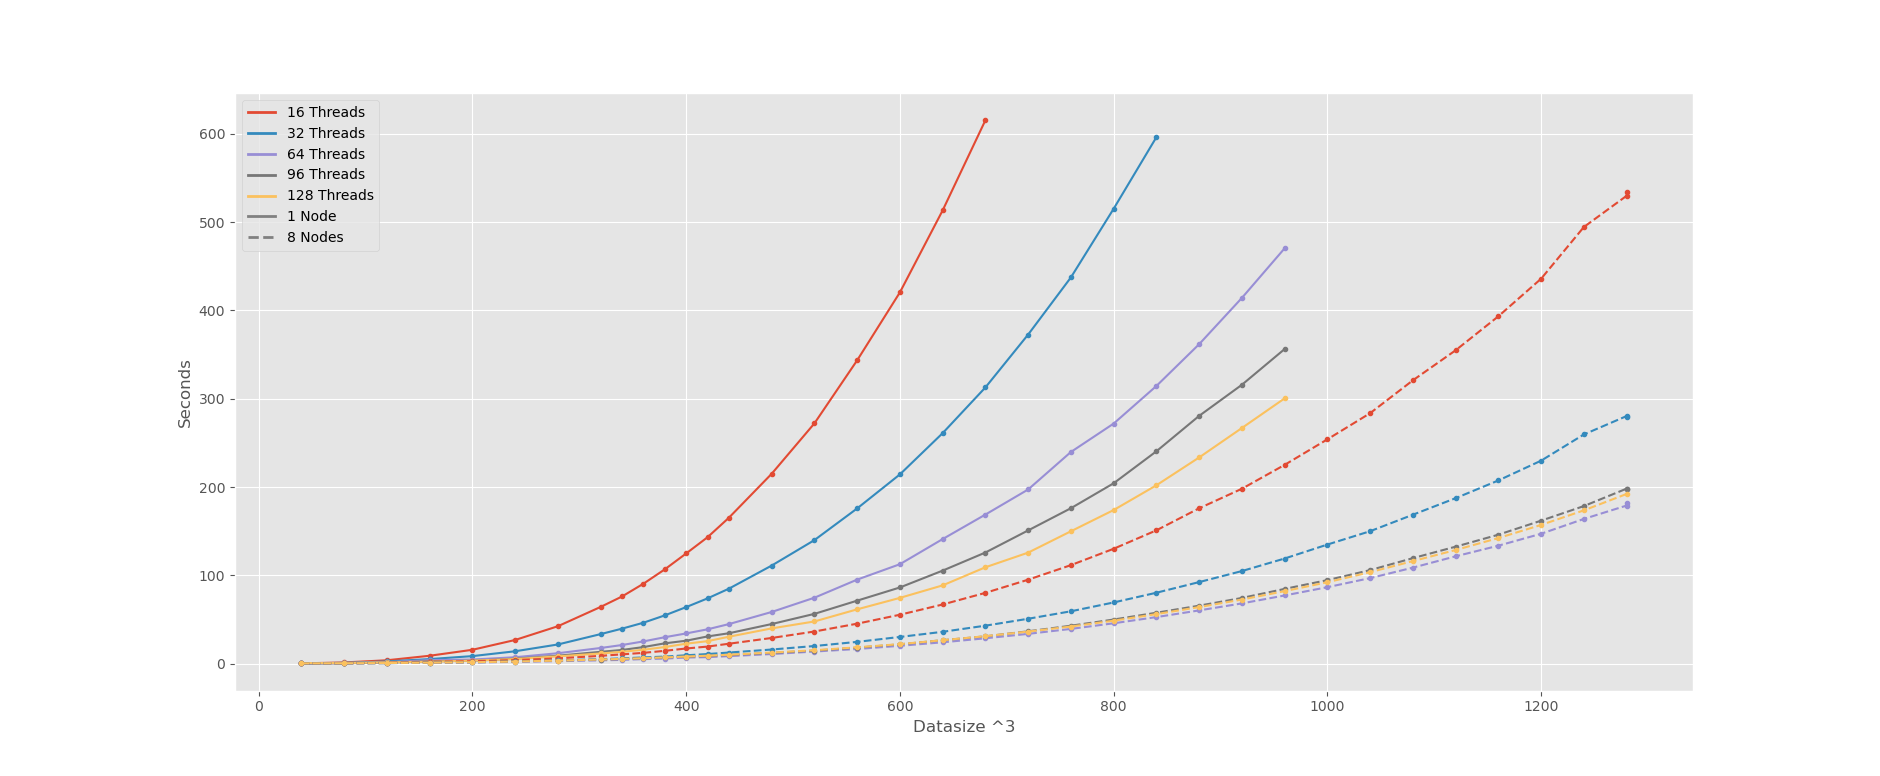
\includegraphics[width=0.9\textwidth]{graphs/boltzmansmp.png}
	\caption{\ac{cpu} Runtimes of the \ac{lbm} \ac{muesli} program}\label{fig1}
\end{figure}

\section{Blur Example}
\begin{figure}[h]%
	\centering
	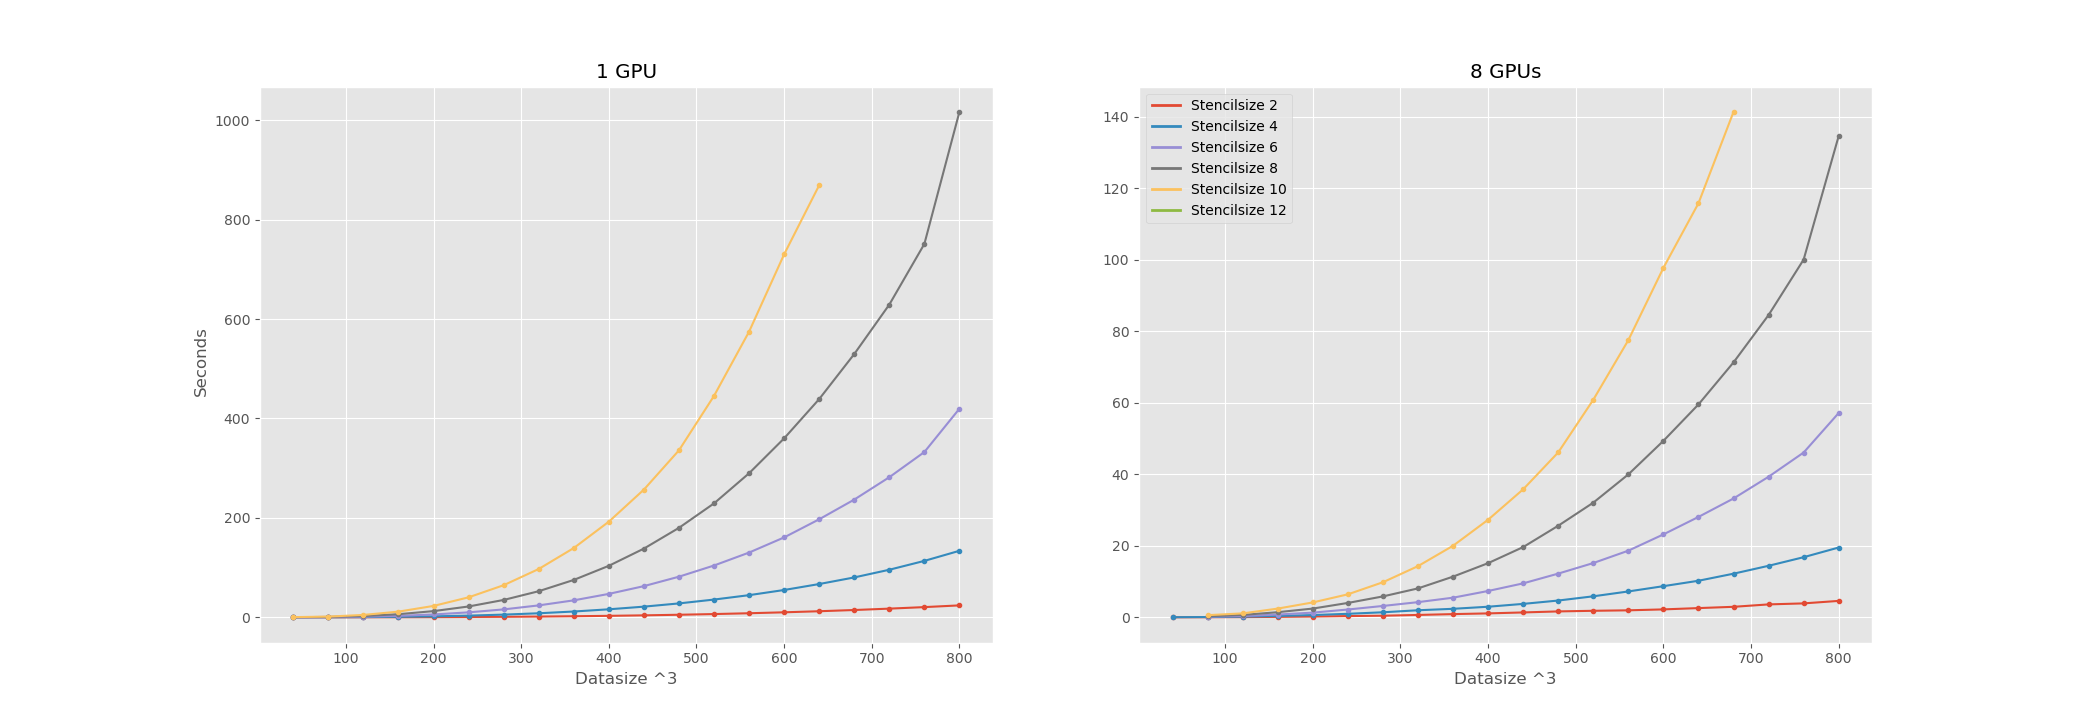
\includegraphics[width=0.9\textwidth]{graphs/blurhgx.png}
	\caption{Runtimes of the Blur \ac{muesli} program on A100 \acp{gpu}}\label{fig1}
\end{figure}

\begin{figure}[h]%
	\centering
	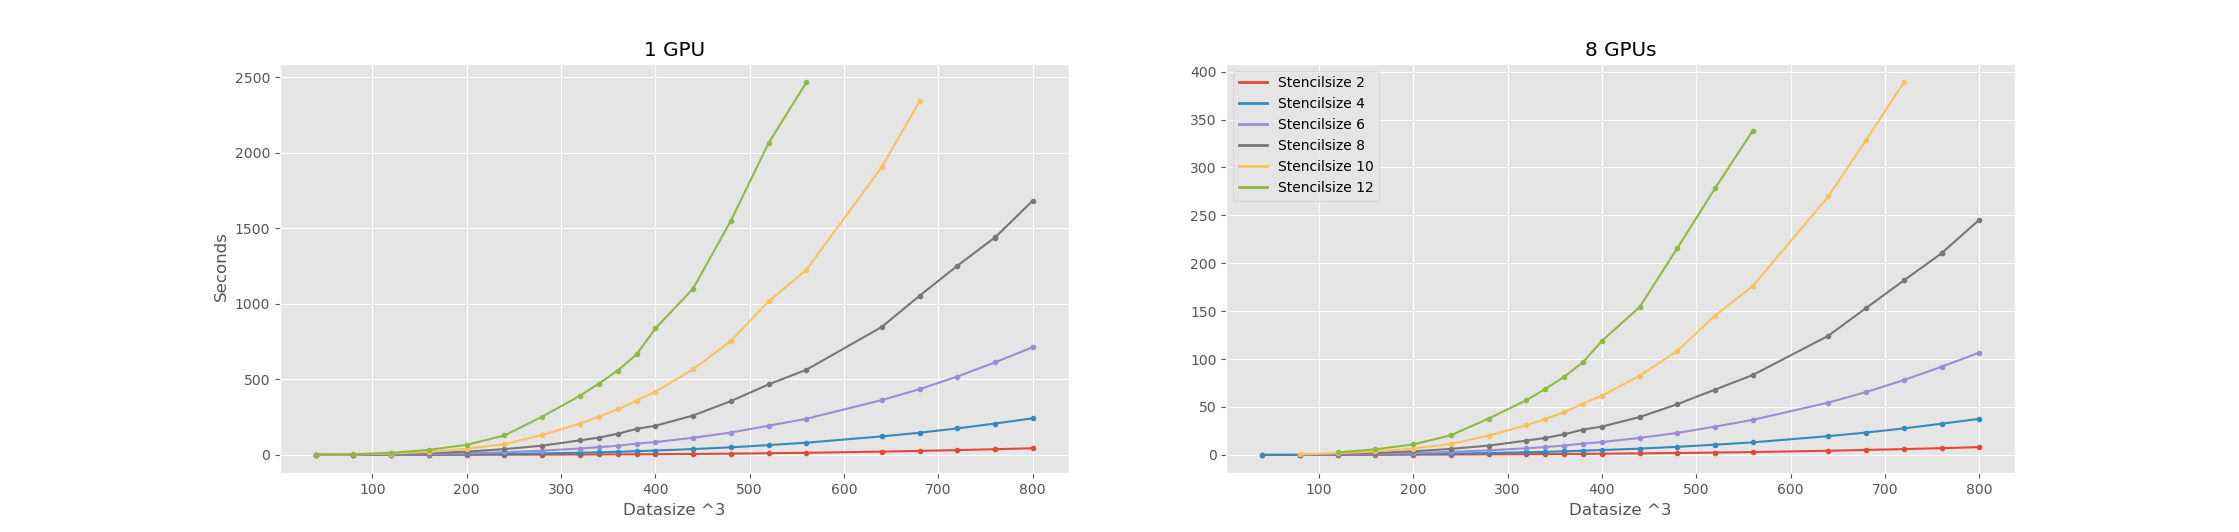
\includegraphics[width=0.9\textwidth]{graphs/gaussian1node2080.png}
	\caption{Runtimes of the Blur \ac{muesli} program on a GeForce RTX 2080 Ti \acp{gpu}}\label{fig1}
\end{figure}
\begin{table}
	\resizebox{\textwidth}{!}{
		\begin{tabular}{r|r||rr|rr|r|r|rr|r|r} \toprule
		blur&	Datasize $^3$ &1 N&1 N-Com&4 Ns&4 Ns -Com&Speed-up&Speed-up&8 Ns&8 Ns -Com&Speed-up&Speed-up\\ \midrule
			\multirow{4}{*}{2}&120&0.16&0.16&0.07&0.05&2.1&3.41&0.09&0.03&1.76&5.56 \\ 
			&280&1.5&1.5&0.58&0.42&2.6&3.55&0.55&0.23&2.74&6.55 \\ 
			&400&4.46&4.46&1.44&1.15&3.09&3.89&1.24&0.61&3.61&7.33 \\ 
			&560&13.56&13.56&3.99&3.4&3.4&3.99&2.95&1.76&4.59&7.71\\    \midrule 
			\multirow{4}{*}{8}&120&4.54&4.54&1.47&1.35&3.09&3.35&1.04&0.79&4.37&5.74\\ 
			&280&60.58&60.58&16.44&15.85&3.68&3.82&9.71&8.47&6.24&7.15\\ 
			&400&192.61&192.61&51.59&50.34&3.73&3.83&29.52&26.96&6.52&7.14\\ 
			&560&563.2&563.2&148.68&146.41&3.79&3.85&83.38&78.58&6.75&7.17\\   \midrule 
			\multirow{4}{*}{12}&120&13.59&13.59&4.2&4.03&3.23&3.37&2.53&2.17&5.38&6.27\\ 
			&280&252.54&252.54&69.24&68.32&3.65&3.7&37.92&35.97&6.66&7.02\\ 
			&400&836.59&836.58&222.12&220.38&3.77&3.8&118.89&115.15&7.04&7.27\\ 
			&560&2464.76&2464.76&643.33&640.16&3.83&3.85&338.46&331.65&7.28&7.43\\   
			\botrule
	\end{tabular}}
	\caption{Speed-up for the Parallel Implementation of the \ac{lbm} Gas Simulation for single \ac{gpu} Programs}
	\label{tab:speedupsinglelbm}
\end{table}
\begin{figure}[h]%
	\centering
	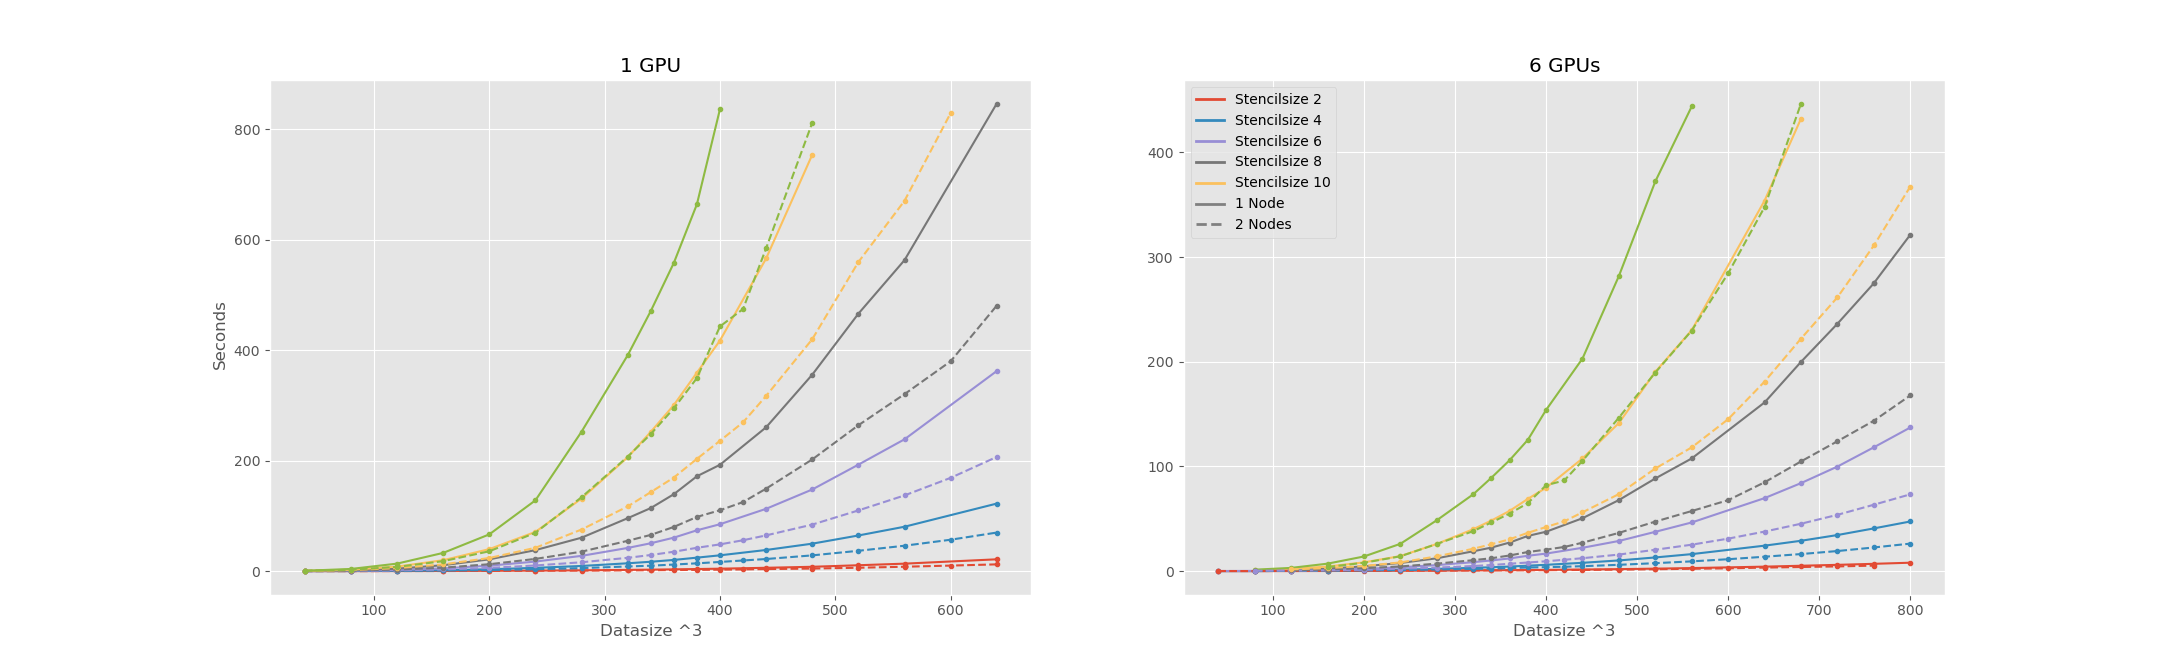
\includegraphics[width=0.9\textwidth]{graphs/blurmnode.png}
	\caption{Runtimes of the Blur \ac{muesli} program on multiple GeForce RTX 2080 Ti \acp{gpu}}\label{fig1}
\end{figure}

\section{Conclusion}\label{sec:conclusion}





%%%%%%%%%%%%%%%%%%%%%%%%%%%%%%%%%%%%%%%% TEMPLATE %%%%%%%%%%%%%%%%%%%%%%%%%%%%%%%%%%%%%%%%%%%%%%%%%%%%%%%%%%%%
Equations in \LaTeX\ can either be inline or on-a-line by itself (``display equations''). For
inline equations use the \verb+$...$+ commands. E.g.: The equation
$H\psi = E \psi$ is written via the command \verb+$H \psi = E \psi$+.

For display equations (with auto generated equation numbers)
one can use the equation or align environments:
\begin{equation}
	\|\tilde{X}(k)\|^2 \leq\frac{\sum\limits_{i=1}^{p}\left\|\tilde{Y}_i(k)\right\|^2+\sum\limits_{j=1}^{q}\left\|\tilde{Z}_j(k)\right\|^2 }{p+q}.\label{eq1}
\end{equation}
where,
\begin{align}
	D_\mu &=  \partial_\mu - ig \frac{\lambda^a}{2} A^a_\mu \nonumber \\
	F^a_{\mu\nu} &= \partial_\mu A^a_\nu - \partial_\nu A^a_\mu + g f^{abc} A^b_\mu A^a_\nu \label{eq2}
\end{align}
Notice the use of \verb+\nonumber+ in the align environment at the end
of each line, except the last, so as not to produce equation numbers on
lines where no equation numbers are required. The \verb+\label{}+ command
should only be used at the last line of an align environment where
\verb+\nonumber+ is not used.
\begin{equation}
	Y_\infty = \left( \frac{m}{\textrm{GeV}} \right)^{-3}
	\left[ 1 + \frac{3 \ln(m/\textrm{GeV})}{15}
	+ \frac{\ln(c_2/5)}{15} \right]
\end{equation}
The class file also supports the use of \verb+\mathbb{}+, \verb+\mathscr{}+ and
\verb+\mathcal{}+ commands. As such \verb+\mathbb{R}+, \verb+\mathscr{R}+
and \verb+\mathcal{R}+ produces $\mathbb{R}$, $\mathscr{R}$ and $\mathcal{R}$
respectively (refer Subsubsection~\ref{subsubsec2}).

Tables can be inserted via the normal table and tabular environment. To put
footnotes inside tables you should use \verb+\footnotetext[]{...}+ tag.
The footnote appears just below the table itself (refer Tables~\ref{tab1} and \ref{tab2}). 
For the corresponding footnotemark use \verb+\footnotemark[...]+

\begin{table}[h]
\caption{Caption text}\label{tab1}%
\begin{tabular}{@{}llll@{}}
\toprule
Column 1 & Column 2  & Column 3 & Column 4\\
\midrule
row 1    & data 1   & data 2  & data 3  \\
row 2    & data 4   & data 5\footnotemark[1]  & data 6  \\
row 3    & data 7   & data 8  & data 9\footnotemark[2]  \\
\botrule
\end{tabular}
\footnotetext{Source: This is an example of table footnote. This is an example of table footnote.}
\footnotetext[1]{Example for a first table footnote. This is an example of table footnote.}
\footnotetext[2]{Example for a second table footnote. This is an example of table footnote.}
\end{table}

\noindent
The input format for the above table is as follows:

%%=============================================%%
%% For presentation purpose, we have included  %%
%% \bigskip command. please ignore this.       %%
%%=============================================%%
\bigskip
\begin{verbatim}
\begin{table}[<placement-specifier>]
\caption{<table-caption>}\label{<table-label>}%
\begin{tabular}{@{}llll@{}}
\toprule
Column 1 & Column 2 & Column 3 & Column 4\\
\midrule
row 1 & data 1 & data 2	 & data 3 \\
row 2 & data 4 & data 5\footnotemark[1] & data 6 \\
row 3 & data 7 & data 8	 & data 9\footnotemark[2]\\
\botrule
\end{tabular}
\footnotetext{Source: This is an example of table footnote. 
This is an example of table footnote.}
\footnotetext[1]{Example for a first table footnote.
This is an example of table footnote.}
\footnotetext[2]{Example for a second table footnote. 
This is an example of table footnote.}
\end{table}
\end{verbatim}
\bigskip
%%=============================================%%
%% For presentation purpose, we have included  %%
%% \bigskip command. please ignore this.       %%
%%=============================================%%

\begin{table}[h]
\caption{Example of a lengthy table which is set to full textwidth}\label{tab2}
\begin{tabular*}{\textwidth}{@{\extracolsep\fill}lcccccc}
\toprule%
& \multicolumn{3}{@{}c@{}}{Element 1\footnotemark[1]} & \multicolumn{3}{@{}c@{}}{Element 2\footnotemark[2]} \\\cmidrule{2-4}\cmidrule{5-7}%
Project & Energy & $\sigma_{calc}$ & $\sigma_{expt}$ & Energy & $\sigma_{calc}$ & $\sigma_{expt}$ \\
\midrule
Element 3  & 990 A & 1168 & $1547\pm12$ & 780 A & 1166 & $1239\pm100$\\
Element 4  & 500 A & 961  & $922\pm10$  & 900 A & 1268 & $1092\pm40$\\
\botrule
\end{tabular*}
\footnotetext{Note: This is an example of table footnote. This is an example of table footnote this is an example of table footnote this is an example of~table footnote this is an example of table footnote.}
\footnotetext[1]{Example for a first table footnote.}
\footnotetext[2]{Example for a second table footnote.}
\end{table}

\vfill\eject

In case of double column layout, tables which do not fit in single column width should be set to full text width. For this, you need to use \verb+\begin{table*}+ \verb+...+ \verb+\end{table*}+ instead of \verb+\begin{table}+ \verb+...+ \verb+\end{table}+ environment. Lengthy tables which do not fit in textwidth should be set as rotated table. For this, you need to use \verb+\begin{sidewaystable}+ \verb+...+ \verb+\end{sidewaystable}+ instead of \verb+\begin{table*}+ \verb+...+ \verb+\end{table*}+ environment. This environment puts tables rotated to single column width. For tables rotated to double column width, use \verb+\begin{sidewaystable*}+ \verb+...+ \verb+\end{sidewaystable*}+.

\begin{sidewaystable}
\caption{Tables which are too long to fit, should be written using the ``sidewaystable'' environment as shown here}\label{tab3}
\begin{tabular*}{\textheight}{@{\extracolsep\fill}lcccccc}
\toprule%
& \multicolumn{3}{@{}c@{}}{Element 1\footnotemark[1]}& \multicolumn{3}{@{}c@{}}{Element\footnotemark[2]} \\\cmidrule{2-4}\cmidrule{5-7}%
Projectile & Energy	& $\sigma_{calc}$ & $\sigma_{expt}$ & Energy & $\sigma_{calc}$ & $\sigma_{expt}$ \\
\midrule
Element 3 & 990 A & 1168 & $1547\pm12$ & 780 A & 1166 & $1239\pm100$ \\
Element 4 & 500 A & 961  & $922\pm10$  & 900 A & 1268 & $1092\pm40$ \\
Element 5 & 990 A & 1168 & $1547\pm12$ & 780 A & 1166 & $1239\pm100$ \\
Element 6 & 500 A & 961  & $922\pm10$  & 900 A & 1268 & $1092\pm40$ \\
\botrule
\end{tabular*}
\footnotetext{Note: This is an example of table footnote this is an example of table footnote this is an example of table footnote this is an example of~table footnote this is an example of table footnote.}
\footnotetext[1]{This is an example of table footnote.}
\end{sidewaystable}


As per the \LaTeX\ standards you need to use eps images for \LaTeX\ compilation and \verb+pdf/jpg/png+ images for \verb+PDFLaTeX+ compilation. This is one of the major difference between \LaTeX\ and \verb+PDFLaTeX+. Each image should be from a single input .eps/vector image file. Avoid using subfigures. The command for inserting images for \LaTeX\ and \verb+PDFLaTeX+ can be generalized. The package used to insert images in \verb+LaTeX/PDFLaTeX+ is the graphicx package. Figures can be inserted via the normal figure environment as shown in the below example:

%%=============================================%%
%% For presentation purpose, we have included  %%
%% \bigskip command. please ignore this.       %%
%%=============================================%%
\bigskip
\begin{verbatim}
\begin{figure}[<placement-specifier>]
\centering
\includegraphics{<eps-file>}
\caption{<figure-caption>}\label{<figure-label>}
\end{figure}
\end{verbatim}
\bigskip
%%=============================================%%
%% For presentation purpose, we have included  %%
%% \bigskip command. please ignore this.       %%
%%=============================================%%

In case of double column layout, the above format puts figure captions/images to single column width. To get spanned images, we need to provide \verb+\begin{figure*}+ \verb+...+ \verb+\end{figure*}+.

For sample purpose, we have included the width of images in the optional argument of \verb+\includegraphics+ tag. Please ignore this. 

\section{Algorithms, Program codes and Listings}\label{sec7}

Packages \verb+algorithm+, \verb+algorithmicx+ and \verb+algpseudocode+ are used for setting algorithms in \LaTeX\ using the format:

%%=============================================%%
%% For presentation purpose, we have included  %%
%% \bigskip command. please ignore this.       %%
%%=============================================%%
\bigskip
\begin{verbatim}
\begin{algorithm}
\caption{<alg-caption>}\label{<alg-label>}
\begin{algorithmic}[1]
. . .
\end{algorithmic}
\end{algorithm}
\end{verbatim}
\bigskip
%%=============================================%%
%% For presentation purpose, we have included  %%
%% \bigskip command. please ignore this.       %%
%%=============================================%%

You may refer above listed package documentations for more details before setting \verb+algorithm+ environment. For program codes, the ``verbatim'' package is required and the command to be used is \verb+\begin{verbatim}+ \verb+...+ \verb+\end{verbatim}+. 

Similarly, for \verb+listings+, use the \verb+listings+ package. \verb+\begin{lstlisting}+ \verb+...+ \verb+\end{lstlisting}+ is used to set environments similar to \verb+verbatim+ environment. Refer to the \verb+lstlisting+ package documentation for more details.

A fast exponentiation procedure:

\lstset{texcl=true,basicstyle=\small\sf,commentstyle=\small\rm,mathescape=true,escapeinside={(*}{*)}}
\begin{lstlisting}
begin
  for $i:=1$ to $10$ step $1$ do
      expt($2,i$);  
      newline() od                (*\textrm{Comments will be set flush to the right margin}*)
where
proc expt($x,n$) $\equiv$
  $z:=1$;
  do if $n=0$ then exit fi;
     do if odd($n$) then exit fi;                 
        comment: (*\textrm{This is a comment statement;}*)
        $n:=n/2$; $x:=x*x$ od;
     { $n>0$ };
     $n:=n-1$; $z:=z*x$ od;
  print($z$). 
end
\end{lstlisting}

\begin{algorithm}
\caption{Calculate $y = x^n$}\label{algo1}
\begin{algorithmic}[1]
\Require $n \geq 0 \vee x \neq 0$
\Ensure $y = x^n$ 
\State $y \Leftarrow 1$
\If{$n < 0$}\label{algln2}
        \State $X \Leftarrow 1 / x$
        \State $N \Leftarrow -n$
\Else
        \State $X \Leftarrow x$
        \State $N \Leftarrow n$
\EndIf
\While{$N \neq 0$}
        \If{$N$ is even}
            \State $X \Leftarrow X \times X$
            \State $N \Leftarrow N / 2$
        \Else[$N$ is odd]
            \State $y \Leftarrow y \times X$
            \State $N \Leftarrow N - 1$
        \EndIf
\EndWhile
\end{algorithmic}
\end{algorithm}

%%=============================================%%
%% For presentation purpose, we have included  %%
%% \bigskip command. please ignore this.       %%
%%=============================================%%
\bigskip
\begin{minipage}{\hsize}%
\lstset{frame=single,framexleftmargin=-1pt,framexrightmargin=-17pt,framesep=12pt,linewidth=0.98\textwidth,language=pascal}% Set your language (you can change the language for each code-block optionally)
%%% Start your code-block
\begin{lstlisting}
for i:=maxint to 0 do
begin
{ do nothing }
end;
Write('Case insensitive ');
Write('Pascal keywords.');
\end{lstlisting}
\end{minipage}

\section{Cross referencing}\label{sec8}

Environments such as figure, table, equation and align can have a label
declared via the \verb+\label{#label}+ command. For figures and table
environments use the \verb+\label{}+ command inside or just
below the \verb+\caption{}+ command. You can then use the
\verb+\ref{#label}+ command to cross-reference them. As an example, consider
the label declared for Figure~\ref{fig1} which is
\verb+\label{fig1}+. To cross-reference it, use the command 
\verb+Figure \ref{fig1}+, for which it comes up as
``Figure~\ref{fig1}''. 

To reference line numbers in an algorithm, consider the label declared for the line number 2 of Algorithm~\ref{algo1} is \verb+\label{algln2}+. To cross-reference it, use the command \verb+\ref{algln2}+ for which it comes up as line~\ref{algln2} of Algorithm~\ref{algo1}.

\subsection{Details on reference citations}\label{subsec7}

Standard \LaTeX\ permits only numerical citations. To support both numerical and author-year citations this template uses \verb+natbib+ \LaTeX\ package. For style guidance please refer to the template user manual.

Here is an example for \verb+\cite{...}+: \cite{MPI}. Another example for \verb+\citep{...}+: \citep{MPI}. For author-year citation mode, \verb+\cite{...}+ prints Jones et al. (1990) and \verb+\citep{...}+ prints (Jones et al., 1990).

All cited bib entries are printed at the end of this article: \cite{MPI}, \cite{MPI}, \cite{MPI}.

\section{Examples for theorem like environments}\label{sec10}

For theorem like environments, we require \verb+amsthm+ package. There are three types of predefined theorem styles exists---\verb+thmstyleone+, \verb+thmstyletwo+ and \verb+thmstylethree+ 

%%=============================================%%
%% For presentation purpose, we have included  %%
%% \bigskip command. please ignore this.       %%
%%=============================================%%
\bigskip
\begin{tabular}{|l|p{19pc}|}
\hline
\verb+thmstyleone+ & Numbered, theorem head in bold font and theorem text in italic style \\\hline
\verb+thmstyletwo+ & Numbered, theorem head in roman font and theorem text in italic style \\\hline
\verb+thmstylethree+ & Numbered, theorem head in bold font and theorem text in roman style \\\hline
\end{tabular}
\bigskip
%%=============================================%%
%% For presentation purpose, we have included  %%
%% \bigskip command. please ignore this.       %%
%%=============================================%%

For mathematics journals, theorem styles can be included as shown in the following examples:

\begin{theorem}[Theorem subhead]\label{thm1}
Example theorem text. Example theorem text. Example theorem text. Example theorem text. Example theorem text. 
Example theorem text. Example theorem text. Example theorem text. Example theorem text. Example theorem text. 
Example theorem text. 
\end{theorem}

Sample body text. Sample body text. Sample body text. Sample body text. Sample body text. Sample body text. Sample body text. Sample body text.

\begin{proposition}
Example proposition text. Example proposition text. Example proposition text. Example proposition text. Example proposition text. 
Example proposition text. Example proposition text. Example proposition text. Example proposition text. Example proposition text. 
\end{proposition}

Sample body text. Sample body text. Sample body text. Sample body text. Sample body text. Sample body text. Sample body text. Sample body text.

\begin{example}
Phasellus adipiscing semper elit. Proin fermentum massa
ac quam. Sed diam turpis, molestie vitae, placerat a, molestie nec, leo. Maecenas lacinia. Nam ipsum ligula, eleifend
at, accumsan nec, suscipit a, ipsum. Morbi blandit ligula feugiat magna. Nunc eleifend consequat lorem. 
\end{example}

Sample body text. Sample body text. Sample body text. Sample body text. Sample body text. Sample body text. Sample body text. Sample body text.

\begin{remark}
Phasellus adipiscing semper elit. Proin fermentum massa
ac quam. Sed diam turpis, molestie vitae, placerat a, molestie nec, leo. Maecenas lacinia. Nam ipsum ligula, eleifend
at, accumsan nec, suscipit a, ipsum. Morbi blandit ligula feugiat magna. Nunc eleifend consequat lorem. 
\end{remark}

Sample body text. Sample body text. Sample body text. Sample body text. Sample body text. Sample body text. Sample body text. Sample body text.

\begin{definition}[Definition sub head]
Example definition text. Example definition text. Example definition text. Example definition text. Example definition text. Example definition text. Example definition text. Example definition text. 
\end{definition}

Additionally a predefined ``proof'' environment is available: \verb+\begin{proof}+ \verb+...+ \verb+\end{proof}+. This prints a ``Proof'' head in italic font style and the ``body text'' in roman font style with an open square at the end of each proof environment. 

\begin{proof}
Example for proof text. Example for proof text. Example for proof text. Example for proof text. Example for proof text. Example for proof text. Example for proof text. Example for proof text. Example for proof text. Example for proof text. 
\end{proof}

Sample body text. Sample body text. Sample body text. Sample body text. Sample body text. Sample body text. Sample body text. Sample body text.

\begin{proof}[Proof of Theorem~{\upshape\ref{thm1}}]
Example for proof text. Example for proof text. Example for proof text. Example for proof text. Example for proof text. Example for proof text. Example for proof text. Example for proof text. Example for proof text. Example for proof text. 
\end{proof}

\noindent
For a quote environment, use \verb+\begin{quote}...\end{quote}+
\begin{quote}
Quoted text example. Aliquam porttitor quam a lacus. Praesent vel arcu ut tortor cursus volutpat. In vitae pede quis diam bibendum placerat. Fusce elementum
convallis neque. Sed dolor orci, scelerisque ac, dapibus nec, ultricies ut, mi. Duis nec dui quis leo sagittis commodo.
\end{quote}

Sample body text. Sample body text. Sample body text. Sample body text. Sample body text (refer Figure~\ref{fig1}). Sample body text. Sample body text. Sample body text (refer Table~\ref{tab3}). 

\section{Methods}\label{sec11}

Topical subheadings are allowed. Authors must ensure that their Methods section includes adequate experimental and characterization data necessary for others in the field to reproduce their work. Authors are encouraged to include RIIDs where appropriate. 

\textbf{Ethical approval declarations} (only required where applicable) Any article reporting experiment/s carried out on (i)~live vertebrate (or higher invertebrates), (ii)~humans or (iii)~human samples must include an unambiguous statement within the methods section that meets the following requirements: 

\begin{enumerate}[1.]
\item Approval: a statement which confirms that all experimental protocols were approved by a named institutional and/or licensing committee. Please identify the approving body in the methods section

\item Accordance: a statement explicitly saying that the methods were carried out in accordance with the relevant guidelines and regulations

\item Informed consent (for experiments involving humans or human tissue samples): include a statement confirming that informed consent was obtained from all participants and/or their legal guardian/s
\end{enumerate}

If your manuscript includes potentially identifying patient/participant information, or if it describes human transplantation research, or if it reports results of a clinical trial then  additional information will be required. Please visit (\url{https://www.nature.com/nature-research/editorial-policies}) for Nature Portfolio journals, (\url{https://www.springer.com/gp/authors-editors/journal-author/journal-author-helpdesk/publishing-ethics/14214}) for Springer Nature journals, or (\url{https://www.biomedcentral.com/getpublished/editorial-policies\#ethics+and+consent}) for BMC.

\section{Discussion}\label{sec12}

Discussions should be brief and focused. In some disciplines use of Discussion or `Conclusion' is interchangeable. It is not mandatory to use both. Some journals prefer a section `Results and Discussion' followed by a section `Conclusion'. Please refer to Journal-level guidance for any specific requirements. 

\section{Conclusion}\label{sec13}

Conclusions may be used to restate your hypothesis or research question, restate your major findings, explain the relevance and the added value of your work, highlight any limitations of your study, describe future directions for research and recommendations. 

In some disciplines use of Discussion or 'Conclusion' is interchangeable. It is not mandatory to use both. Please refer to Journal-level guidance for any specific requirements. 

\backmatter

\bmhead{Supplementary information}

If your article has accompanying supplementary file/s please state so here. 

Authors reporting data from electrophoretic gels and blots should supply the full unprocessed scans for key as part of their Supplementary information. This may be requested by the editorial team/s if it is missing.

Please refer to Journal-level guidance for any specific requirements.

\bmhead{Acknowledgments}

Acknowledgments are not compulsory. Where included they should be brief. Grant or contribution numbers may be acknowledged.

Please refer to Journal-level guidance for any specific requirements.

\section*{Declarations}

Some journals require declarations to be submitted in a standardised format. Please check the Instructions for Authors of the journal to which you are submitting to see if you need to complete this section. If yes, your manuscript must contain the following sections under the heading `Declarations':

\begin{itemize}
\item Funding
\item Conflict of interest/Competing interests (check journal-specific guidelines for which heading to use)
\item Ethics approval 
\item Consent to participate
\item Consent for publication
\item Availability of data and materials
\item Code availability 
\item Authors' contributions
\end{itemize}

\noindent
If any of the sections are not relevant to your manuscript, please include the heading and write `Not applicable' for that section. 

%%===================================================%%
%% For presentation purpose, we have included        %%
%% \bigskip command. please ignore this.             %%
%%===================================================%%
\bigskip
\begin{flushleft}%
Editorial Policies for:

\bigskip\noindent
Springer journals and proceedings: \url{https://www.springer.com/gp/editorial-policies}

\bigskip\noindent
Nature Portfolio journals: \url{https://www.nature.com/nature-research/editorial-policies}

\bigskip\noindent
\textit{Scientific Reports}: \url{https://www.nature.com/srep/journal-policies/editorial-policies}

\bigskip\noindent
BMC journals: \url{https://www.biomedcentral.com/getpublished/editorial-policies}
\end{flushleft}

\begin{appendices}

\section{Section title of first appendix}\label{secA1}

An appendix contains supplementary information that is not an essential part of the text itself but which may be helpful in providing a more comprehensive understanding of the research problem or it is information that is too cumbersome to be included in the body of the paper.

%%=============================================%%
%% For submissions to Nature Portfolio Journals %%
%% please use the heading ``Extended Data''.   %%
%%=============================================%%

%%=============================================================%%
%% Sample for another appendix section			       %%
%%=============================================================%%

%% \section{Example of another appendix section}\label{secA2}%
%% Appendices may be used for helpful, supporting or essential material that would otherwise 
%% clutter, break up or be distracting to the text. Appendices can consist of sections, figures, 
%% tables and equations etc.

\end{appendices}

%%===========================================================================================%%
%% If you are submitting to one of the Nature Portfolio journals, using the eJP submission   %%
%% system, please include the references within the manuscript file itself. You may do this  %%
%% by copying the reference list from your .bbl file, paste it into the main manuscript .tex %%
%% file, and delete the associated \verb+\bibliography+ commands.                            %%
%%===========================================================================================%%
%\printbibliography
\bibliography{sn-bibliography}% common bib file
%% if required, the content of .bbl file can be included here once bbl is generated
%%\input sn-article.bbl


\end{document}
